\documentclass[tikz]{standalone}

\usetikzlibrary{calc,positioning,shapes,positioning,intersections,quotes}
\usepackage{amsfonts,amsmath,amsthm,amssymb,mathtools,stmaryrd,mathrsfs}

\begin{document}
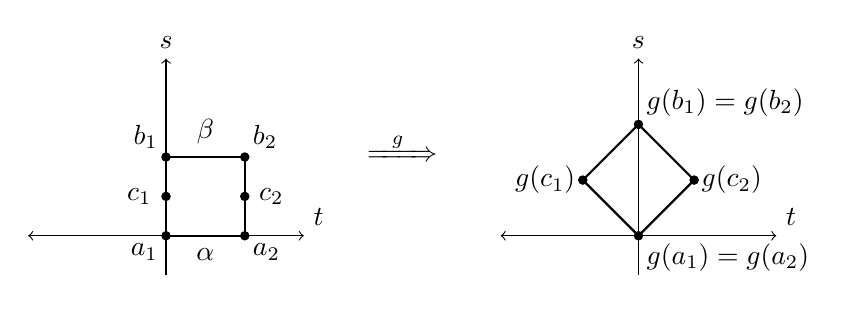
\begin{tikzpicture}
  \draw[->] (0,0) to +(1.75,0) node [above right] {$t$};
  \draw[->] (0,0) to +(0,2.25) node [above] {$s$};

  \draw[->] (0,0) to +(-1.75,0);
  \draw[-] (0,0) to +(0,-0.5);

  \draw [thick] (0,0) -- (0,1) -- (1,1) -- (1,0) -- cycle;
  
  \node [fill, draw, circle, minimum width=3pt, inner sep=0pt] (r) at (0,0) {};
  \node[below left=-0.25em of r] {$a_1$};

  \node [fill, draw, circle, minimum width=3pt, inner sep=0pt] (r) at (1,0) {};
  \node[below right=-0.25em of r] {$a_2$};

  %%

  \node [fill, draw, circle, minimum width=3pt, inner sep=0pt] (r) at (0,1) {};
  \node[above left=-0.25em of r] {$b_1$};

  \node [fill, draw, circle, minimum width=3pt, inner sep=0pt] (r) at (1,1) {};
  \node[above right=-0.25em of r] {$b_2$};

  %%

  \node [fill, draw, circle, minimum width=3pt, inner sep=0pt] (r) at (0,0.5) {};
  \node[left=0em of r] {$c_1$};

  \node [fill, draw, circle, minimum width=3pt, inner sep=0pt] (r) at (1,0.5) {};
  \node[right=0em of r] {$c_2$};

  %%

  \node (r) at (0.5,0){};
  \node[below=-0.25em of r] {$\alpha$};
  \node (r) at (0.5,1){};
  \node[above=-0.25em of r] {$\beta$};

  \node at (3,1) {$\xRightarrow{\ \ g\ \ }$};

  \begin{scope}[shift={(6,0)}]

  \draw[->] (0,0) to +(1.75,0) node [above right] {$t$};
  \draw[->] (0,0) to +(0,2.25) node [above] {$s$};

  \draw[->] (0,0) to +(-1.75,0);
  \draw[-] (0,0) to +(0,-0.5);

  \draw [thick] (0,0) -- ({sqrt(2)/2},{sqrt(2)/2}) -- (0,{sqrt(2)}) -- ({-sqrt(2)/2},{sqrt(2)/2}) -- cycle;

  \node [fill, draw, circle, minimum width=3pt, inner sep=0pt] (r) at (0,0) {};
  \node[below right=-0.25em of r,anchor=north west] {$g(a_1)=g(a_2)$};

  %%

  \node [fill, draw, circle, minimum width=3pt, inner sep=0pt] (r) at (0,{sqrt(2)}) {};
  \node[above right=-0.25em of r,anchor=south west] {$g(b_1)=g(b_2)$};

  %%

  \node [fill, draw, circle, minimum width=3pt, inner sep=0pt] (r) at ({sqrt(2)/2},{sqrt(2)/2}) {};
  \node[right=-0.25em of r] {$g(c_2)$};

  %%

  \node [fill, draw, circle, minimum width=3pt, inner sep=0pt] (r) at ({-sqrt(2)/2},{sqrt(2)/2}) {};
  \node[left=-0.25em of r] {$g(c_1)$};

  \end{scope}

\end{tikzpicture}
\end{document}

